% !Mode:: "TeX:UTF-8"
% !TeX encoding = UTF-8
% !TEX program = pdflatex

\documentclass{mcmthesis}
%\usepackage[UTF8]{CTEX}

%\usepackage{fontspec,xltxtra,xunicode}
%\usepackage[slantfont,boldfont]{xeCJK}
%\setCJKmainfont[BoldFont=Adobe Heiti Std,ItalicFont=Adobe Kaiti Std]{Adobe Song Std}
%\setCJKsansfont{Adobe Heiti Std}
%\setCJKmonofont{Adobe Song Std}

\mcmsetup{CTeX = false,   % 使用 CTeX 套装时,设置为 true
	tcn = {\color{red}67859}, problem = {\color{red}D}
%	        }
	,
	sheet = false, titleinsheet = false, keywordsinsheet = false,
	titlepage = false, abstract = false}
\usepackage{palatino}
\usepackage{enumitem} % Required for manipulating the whitespace between and within lists
\usepackage{listings}
\usepackage{multirow}
\usepackage{nicefrac}
\usepackage{sectsty}
%\sectionfont{\color{MidnightBlue}\selectfont}
%\subsectionfont{\color{MidnightBlue!50!RoyalBlue}\selectfont}
%\subsubsectionfont{\color{SkyBlue!5!RoyalBlue}\selectfont}
\usepackage{booktabs}

\usepackage{varioref} % More descriptive referencing
%\setlength\parindent{0pt}
\usepackage{subfig}

\usepackage[subfigure]{tocloft}
\renewcommand\cftsecfont{\bfseries\textbf{\color{MidnightBlue}}}
%\renewcommand\cftpartpagefont{\color{RoyalBlue}}

%\usepackage[round]{natbib}
\usepackage[square,sort,comma,numbers]{natbib}
%\bibliographystyle{ieeetr}
\bibliographystyle{plainnat}

\usepackage{soul}
\definecolor{Light}{gray}{.90}
\sethlcolor{Light}
\let\OldTexttt\texttt
\renewcommand{\texttt}[1]{\OldTexttt{\hl{#1}}}% will affect all \texttt
%\newcommand{\hltexttt}[1]{\texttt{\hl{#1}}}% comment above \renewcommand if want this

\hypersetup{	unicode=false,          % non-Latin characters in Acrobat’s bookmarks
	pdftoolbar=true,        % show Acrobat’s toolbar?
	pdfmenubar=true,        % show Acrobat’s menu?
	pdffitwindow=false,     % window fit to page when opened
	pdfstartview={FitH},    % fits the width of the page to the window
	pdftitle={AI-hw1},    % title
	pdfauthor={Xinglu Wang},     % author
	pdfsubject={Opinions for AI},   % subject of the document
	pdfcreator={},   % creator of the document
	pdfproducer={}, % producer of the document
	pdfkeywords={}, % list of keywords
	pdfnewwindow=true,      % links in new PDF window
	colorlinks=true,       % false: boxed links; true: colored links
	linkcolor=RoyalBlue,          % color of internal links (change box color with linkbordercolor)
	citecolor=ForestGreen,        % color of links to bibliography
	filecolor=magenta,      % color of file links
	urlcolor=Brown,           % color of external links
%	allcolors=Black,
	bookmarksopen=true,
	breaklinks=true,
	bookmarksnumbered
}

\begin{document}
%		\maketitle
\begin{center}
	\textbf{\LARGE{Artificial Intelligence, Spring 2017}} \\
	\vspace{0.2em}
	\large{Homework 1 -- Thoughts about AI} \\
	\vspace{1em}
	{\itshape Xinglu Wang} \quad {\itshape 3140102282} \quad {\itshape ISEE 1403, ZJU}
\end{center}
%		\tableofcontents
\section{AlphaGo}\label{sec1}
I try to understand the mechanism of AlphaGo\cite{1}. My conclusion/thought is that AlphaGo is powerful but is not mysterious and there is a long way to general AI (Current AI just  act rationally on specific and \textit{isolated} task). Let me give some shallow introductions to AlphaGo.


\subsection{MCTS}
Computer is good at computation, so I think search is \textit{still} the basic key component, while the prediction methods(CNN, SL, RL) are just to improve.
\begin{center}

\begin{tabular}{ll}
	\toprule
	Def. for Go Game & Symbol  \\ 
	\midrule
	state space & $\mathcal{S}$  \\ 
	 
	action space for $s \in \mathcal{S}$& $\mathcal{A}_s$ \\ 
	
	state transitions at step t& $s_{t+1}=f(s_t,a_t)$ \\ 
	 
	reward function at step t & $r(s_t)$  \\
	
	outcome of game at terminal time T & $z_t=\pm r(s_T)$  \\
	\bottomrule 
\end{tabular} 
\end{center}

The traditional method (\textit{minmax} search) define an optimal value function   recursively  and need to expand the tree to the terminal time-step when calculating. 
\begin{equation}\label{eq1}
v^*(s)=\left\{
	\begin{array}{ll}
	z_T & \text{if  } s=s_T\text{,}\\
	\displaystyle \max_a \left(-v^*(f(s,a))\right) & \text{otherwise}
	\end{array}
	\right.
\end{equation}
To calculate optimal value, we observe that \textit{minmax} search involve two steps: 
\begin{itemize}[noitemsep]
	\item If the policy for us and opponent is fixed, we need to calculate expected outcome.
	\item   The policy is taking minmax optimal actions in each step. 	
\end{itemize}

An alternative approach to minimax search is Monte-Carlo tree search (MCTS). Similar to \textit{minmax} search, MCTS make double approximation to get $V^n(s) \approx v^*(s)$: 
\begin{itemize}[noitemsep]
	\item Use $n$ Monte-Carlo simulation to estimate expectation.
	\item Use a  simulation policy to take actions $a_t$ controlled by function: \begin{equation}\label{eq2}
	a_t=\displaystyle {\arg \max_a} (Q^n(s,a)+u(s,a)) 
	\end{equation}
	 In UCT,  $Q^n(s,a)=-V^n(f(s,a))$ and $u(s,a)$ is responsible for encouraging explorations. (I try to understand "encourage explorations" in AlphaGo's method.)
\end{itemize}


AlphaGo is based on MCTS integrated with CNN. There are policy function/network, $p_\sigma$ (accurate) and $p_\pi$ (fast); value function/network $v_\theta$. The eq. \eqref{eq2} is split into two part shown below.

The overall evaluation is evaluated by mixed value network $v_\theta$ and rollout evaluations with weight $\lambda$:
\begin{equation}
	Q(s_t,a_t)=(1-\lambda)v_\theta(f(s_t,a_t)) + \lambda z_t
\end{equation}
The outcome $z_t$ is random rollout outcome follow the fast policy function $p_\pi$ (i.e. $a_t \sim p_\pi(\cdot | s_t)$).

\begin{equation}
	u(s,a)\propto \frac{P(s,a)}{1+N(s,a)}
\end{equation}
Here $P(s,a)=p_\sigma(a|s)$ is the prior probabilities for state/node $s$, calculated by accurate policy network $p_\sigma$. We can explain why $u(s,a)$ "encourage explorations" now: Initially, this search control strategy prefer actions with prior probability and low visit count. But after iterating and updating $Q(s,a)$, it will prefer to actions with high value.

 
To conclude, $u(s,a)$ (concerning $p_\sigma(a|s)$) choose the \textit{local} optimal action while $Q(s_t,a)$ (concerning $v_\theta(f(s_t,a)$) choose the \textit{global} optimal action.


Meanwhile, we can further explain why use(and train) $p_\sigma$, $p_\pi$, and $v_\theta$ rather than others afterwards. Ref. to sec. \ref{sec2}.

%Now AlphaGo regress the optimal value function from the huge datasets generated by Reinforcement Learning (rather than TODO Human Dataset, because TODO). $v^*(s)=v_\theta=f_{CNN}(s;W)$

\subsection{Policy \& Value Network}\label{sec2}
\begin{figure}[]
	\centering
	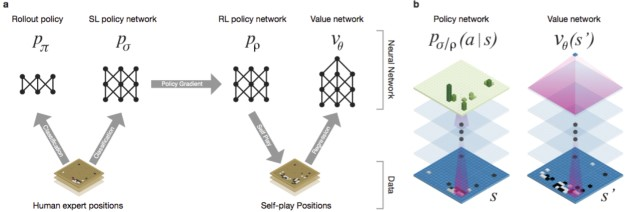
\includegraphics[width=.8\columnwidth]{./fig1.jpg}
	\caption[network]{\textbf{Left}: Neural network training pipeline; \textbf{Right}: Network architecture; 
	\textbf{Note:} $p_{\sigma/\rho}(a|s) $ means $p_\sigma(a|s)$ or $p_\rho(a|s)$}\label{fig1}
\end{figure}
Illustrated in fig. \ref{fig1}, the architecture of $p_\sigma$, $p_\pi$, $p_\rho$, and $v_\theta$ is easy to understand. We just need  to be careful with the notation $p_{\sigma/\rho}(a|s) $, which means  $p_\sigma(a|s)$ \textit{or} $p_\rho(a|s)$, rather than $P_{Y|X}(y|x)$. (As to $p_\rho$, I  need more  time to figure out how to apply \textit{police gradient descent} in Reinforcement Learning). 

$p_\sigma$, $p_\pi$ are trained by SL(classification), $p_\rho$ is trained by RL and $v_\theta$ is trained by SL(regression). 
\begin{itemize}
	\item $p_\pi$ composed with linear units and hand-crafted feature, with less accuracy and fast speed, is proper for rollout search.
	\item $p_\sigma$ trained on Human expert datasets, learn rules of Go and have more diverse choose than $p_\rho$, thus used in initialize prior probabilities.
	\item $v_\theta$ trained on huge generated datasets, have a good sense of global optimal intuition.  
\end{itemize}
This two modules trained on such huge datasets, and only achieve Amateur dan if not combined with MCTS. Meanwhile they cannot generalize to other tasks. Thus, these modules are not so clever as human and there is a long way to go.

%\section{History of AI}

\section{My Opinions}
Conclude from sec. \ref{sec1} and \cite{2}, my opinions are: 
\begin{itemize}
	\item  The mathematics principle behind Search and Reinforcement Learning are quite interesting. Some ideas behind  the algorithms in AI are delicate.  I am looking forward to learn AI systematically!
	\item As stated in AlphaGO (sec. \ref{sec1}), CNN help AI form some intuition about global optimum. But I do not think it is the intuition  human have, because it needs so much training data, still limited in isolated task and cannot transfer to other domain. There is a long run to go, and as researchers, we just try to improve it. 
	\item People are crazy about AI, but we should keep calm, try to figure out why some algorithms in AI perform so good and try to form more delicate idea.
\end{itemize}		
\begin{thebibliography}{99}
\bibitem{1} Silver, David, et al. "Mastering the game of Go with deep neural networks and tree search." Nature 529.7587 (2016): 484-489.
Publishing Company , 1984-1986.
\bibitem{2} \url{https://www.quora.com/Are-neural-networks-the-future-of-AI}
\bibitem{3} \url{https://youtu.be/yCALyQRN3hw?list=PLqYmG7hTraZA7v9Hpbps0QNmJC4L1NE3S&t=11434}

\end{thebibliography}	
	
\end{document}
